\chapter{Postup}
\label{5-postup}

\section{Aktualizace pluginu do verze 1.0.0}
Po dokončení pluginu v předmětu Free Software GIS měl plugin veškerou základní 
funkcionalitu, kterou měl mít. Tou bylo načítání GTFS ZIP souboru do QGISu,
rozbalení ZIP souboru, načtení CSV souborů do geodatabázového kontajneru GeoPackage,
vytvoření vektorových vrstev pro soubory \textit{stops.txt} a \textit{shapes.txt},
obarvení vektorové vrty \textit{shapes.txt} a vložení do CSV souborů a vrstev do
\textit{layer tree}.
% vysvětlit layer tree, GeoPackage??

Avšak pro uvedení do "ostrého" provozu musel být plugin více uživatelsky přívětivější.
Proto byl veškerý proces přesunut na pozadí, aby celý QGIS program "nezamrzal" a
mohla se při jeho výpočtech provádět i jiné akce. To se provedlo díky python třídě \textit{QgsTask}
a jejím metodám, které byly zděděny z této třídy. \cite{QgsTask}
% dát sem i ukázku kódu? 

Pro zobrazování procesu během výpočtu byla použita třída \textit{QProgressBar} a její metody.
Zobrazení postupu bylo implementováno do lišty zpráv QGISu spolu s chybovými hláškami.

\begin{figure}[H] \centering
    
\includegraphics[width=400pt]{./pictures/loading.png}
    \caption[ProgressBar]{ProgressBar v liště QGISu}
	\label{fig:ProgressBar v liště QGISu}              
\end{figure}     

% možná přidat code refactorization

\section{Postup 1 - pomocí nástrojů QGIS}

GTFS obsahuje povinný CSV soubor \textit{stops.txt}. Tento soubor obsahuje mimo
jiných polí také pole \textit{zone\_id}, které bylo při tvorbě tarifních pásem klíčové. 
Pole \textit{zone\_id} má datový typ \textit{string} a znamená, ve kterém tarifním
pásmu daná zastávka leží. Verze GTFS Loaderu 1.0.0 soubor \textit{stops.txt} převádí do vektorové vrstvy
ve formě bodů. Z této bodové vrstvy byla vytvořena vektorová vrstva Voroného 
diagramů nástrojem \textit{Voroného polygony} v programu QGIS. 

Pro použití QGIS nástrojů v pythoním skriptu je potřeba importovat modul \textit{processing},
který má funkci \textit{run}, do které se vkládají dva parametry. První parametr je ID nástroje
ve formě \textit{stringu} a druhý je \textit{slovník} vstupních parametrů. Vstupní parametry se lze dozvědět
z QGIS dokumentace. \cite{QGIS_docs}

Vstupem do tohoto nástroje je vektorová vrstva stops a výstupem jsou právě Voroného polygony.

%toto možná dát do teoretické části
Voroného diagramy, někdy pod názvy jako Voroného teselace, Voroného dekompozice,
Thiessenovy polygony nebo Dirichletova teselace, podle definice představují
rozklad množiny bodů \textit{P} na \textit{n} uzavřených či 
otevřených oblastí \textit{V(p) = \{V(p\textsubscript{i}), V(p\textsubscript{2}), ...,
V(p\textsubscript{n})\}} takových, že každý bod
\textit{q} nálěžící množině \textit{V(p\textsubscript{i})} je blíže k bodu
\textit{p\textsubscript{i}} než k jakémukoliv
bodu \textit{p\textsubscript{j}} náležící množině \textit{P}. \cite{bayer}

\begin{figure}[H] \centering
    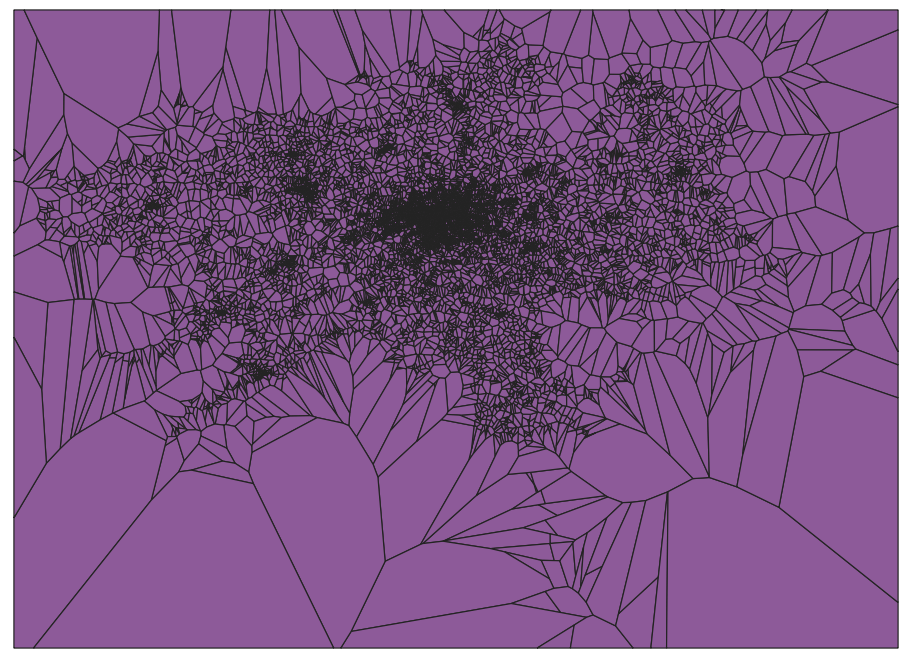
\includegraphics[width=400pt]{./pictures/voronoi.png}
    \caption[Voroného polygony]{Voroného polygony}
	\label{fig:voronoi}              
\end{figure}     

\subsubsection{Vlastnosti Voroného diagramů}

\begin{itemize}
\item Voronoi diagram \textit{V(P)} je planárním grafem.
\item Vrchol q Voronoi buňky \textit{\{V(p\textsubscript{i})} je průnikem 3 hran, právě když je \textit{V(P)} nedegenerovaný.
\item Pokud \textit{p\textsubscript{i}} náležící \textit{H(P)}, pak je \textit{V(p\textsubscript{i})}  otevřený. 
\item Pro každý bod \textit{p\textsubscript{i} náležící P} je \textit{V(P)} konvexní. 
\item Bod \textit{p\textsubscript{i}} je nejbližším bodem bodu \textit{p}
jestliže \textit{p} náleží \textit{\{V(p\textsubscript{i})}.
%nerovnitko? 
\item Každá strana \textit{q\textsubscript{i}q\textsubscript{j}}, \textit{i se nerovná j},
je sdílena právě dvěma sousedními buňkami \textit{V(p)}. 
\item Bod q je vrcholem \textit{V(p)}, pokud existuje kružnice \textit{k(q,r)} procházející třemi
nebo více generátory \textit{p\textsubscript{i}}, \textit{p\textsubscript{j}},
\textit{p\textsubscript{k}}, a neobsahuje žádný další bod P (spojitost s \textit{DT(P)}). 
\item Kružnici \textit{k(q,r)} označujeme jako největší prázdnou kružnici ze všech prázdných kružnic se středem v bodě \textit{q}. 
\item Průměrné množství Voronoi hran ve Voronoi polygonu nepřekročí hodnotu 6. 
\item Vztah mezi počtem bodů \textit{n}, počtem hran \textit{n\textsubscript{h}}
a počtem trojúhelníků \textit{n\textsubscript{t}} teselace \textit{V(P)}:

\[ n_h \leq 3n-6\]
%zjistit, jak se přidat dva vzorce pod sebe
%\[ n_t \leq 2n−5\]

\item Voronoi diagram \textit{V(P)} představuje ortografickou projekci stěn
mnohostěnu tvořeného průsečnicemi všech polorovin \textit{A\textsubscript{i}} do roviny \textit{xy}. 
\item Nechť bod \textit{p\textsubscript{i}\textsuperscript{*}} i představuje
ortografický průmět bodu \textit{p\textsubscript{i}} na povrch paraboloidu daného rovnicí:
\[ z = x^2 + y^2 \]
   
\end{itemize} 

\begin{figure}[H] \centering
    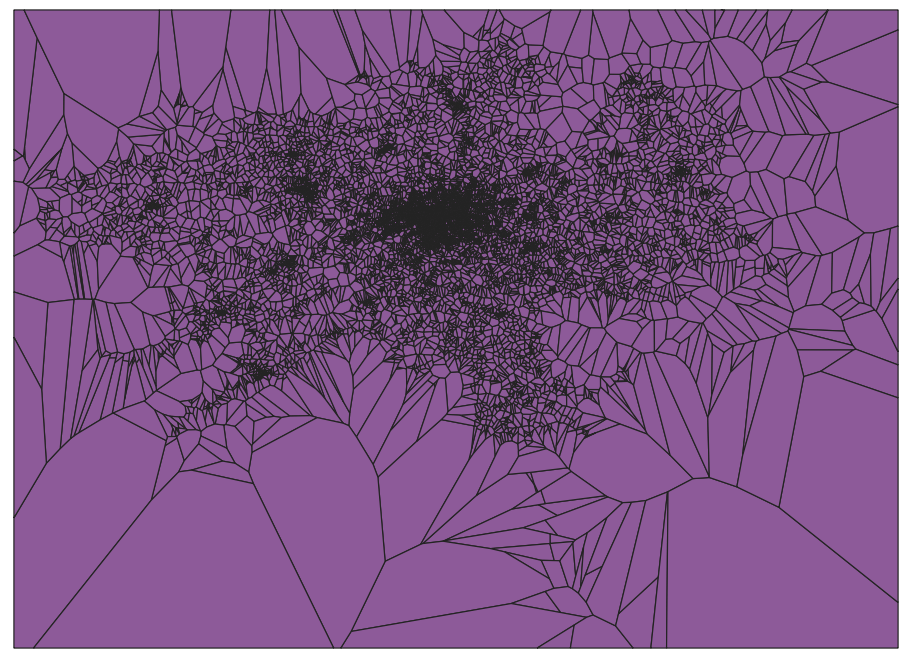
\includegraphics[width=400pt]{./pictures/voronoi-stops.png}
    \caption[Voroného polygony pro všechny zastávky]{Voroného polygony pro všechny zastávky}
	\label{fig:voronoi-stops}              
\end{figure}
  
Pro každé tarifní pásmo byly vybrány zastávky pomocí třídy \textit{QgsVectorLayer}
a její metody \textit{selectByExpression}, která vybírá prvky podle zadaného výrazu ve formě \textit{string}.
Znění zadaného výrazu je následující:

%zjistit, jak lépe přidat části kódu
\textit{zone\_id in "tarifní pásmo" and location\_type = 0}

V zadávaném výrazu figuruje taktéž údaj o poli \textit{location\_type}, což je typ lokace. 
Hodnota nuly (nebo prázdná hodnota) je právě lokace zastávky. 
Třída \textit{QgsVectorLayer} představuje zároveň vektorovou vrstvu, která spravuje
vektorové datové sady a která může být považována jako vstup do nástroje QGIS. % tim chci rict, ze do vstupu nemuze jit string, tzn pouha cesta k vrstve

Pro vybrané zástavky bylo potřeba vybrat ty Voroného polygony, které svou
pozicí dané zastávky protínaly. To bylo provedeno nástrojem \textit{Select by location},
do kterého vstupovala vrstva vybraných zastávek a vrstva Voroného polygonů. Výsledkem tohoto nástroje byla
vektorová vrstva vybraných Voroného polygonů. Jako příklad v obrázku zde budu uvádět tarifní pásmo 2.

\begin{figure}[H] \centering
    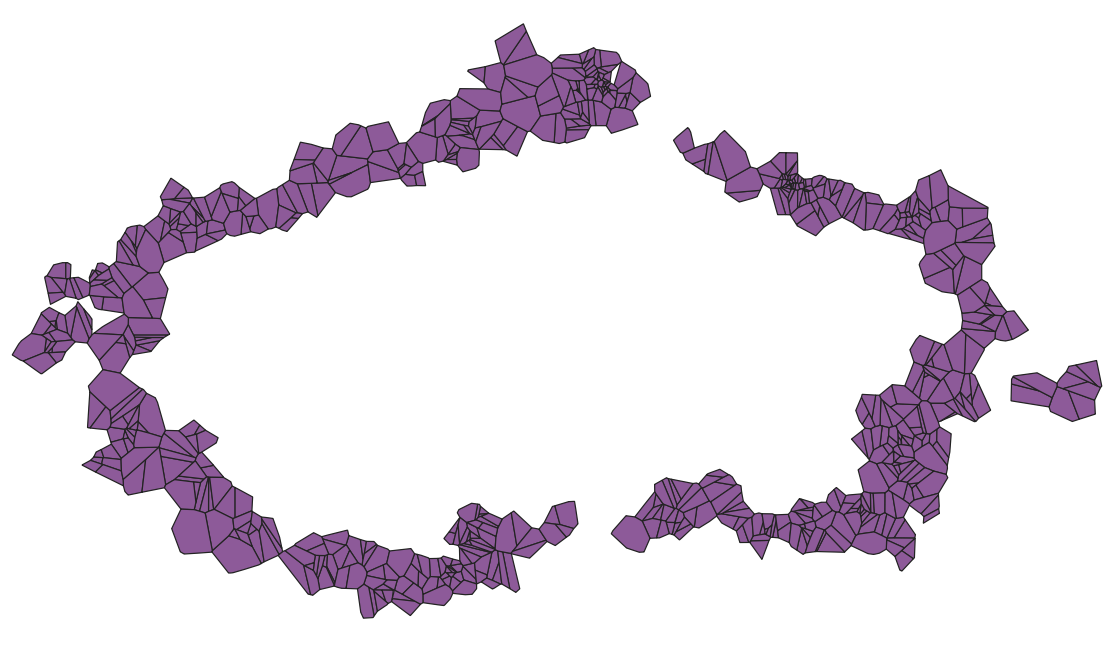
\includegraphics[width=400pt]{./pictures/voronoi-selected.png}
    \caption[Vybrané Voroného polygony pro pásmo 2]{Vybrané Voroného polygony pro pásmo 2}
	\label{fig:voronoi-selected}              
\end{figure}

Tyto polygony byly následně nástrojem \textit{Dissolve} spojeny do jednoho společného polygonu.
Vstupem tohoto nástroje byl výstup nástroje \textit{Select by location} a výstupem byl polygon
s jednou geometrií. 

\begin{figure}[H] \centering
    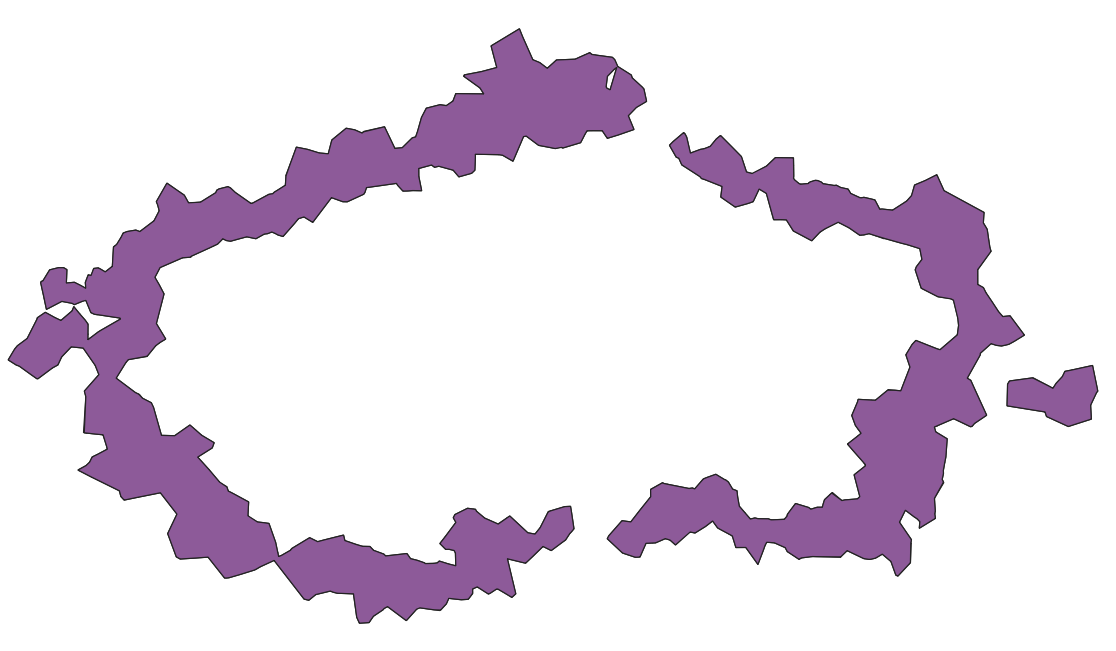
\includegraphics[width=400pt]{./pictures/dissolve.png}
    \caption[Výsledek nástroje Dissolve pro pásmo 2]{Výsledek nástroje Dissolve pro pásmo 2}
	\label{fig:dissolve}              
\end{figure} 

Ze spojených polygonů byla poté vygenerována vektorová vrstva bodů nástrojem
\textit{Extract vertices}, která představovala vrcholy spojených polygonů. Pro tuto vrstvu
bylo vstupem výstup nástroje \textit{Dissolve} a výstupem byl vektorová vrstva bodů 
doplněná o pole (mimo původních polí z vektorové vrstvy \textit{stops}) jako \textit{vertex\_index,
vertex\_part, vertex\_part\_ring, distance} a \textit{angle}.
Hodnoty těchto polí avšak nebyly využity v dalším výpočtu.

\begin{figure}[H] \centering
    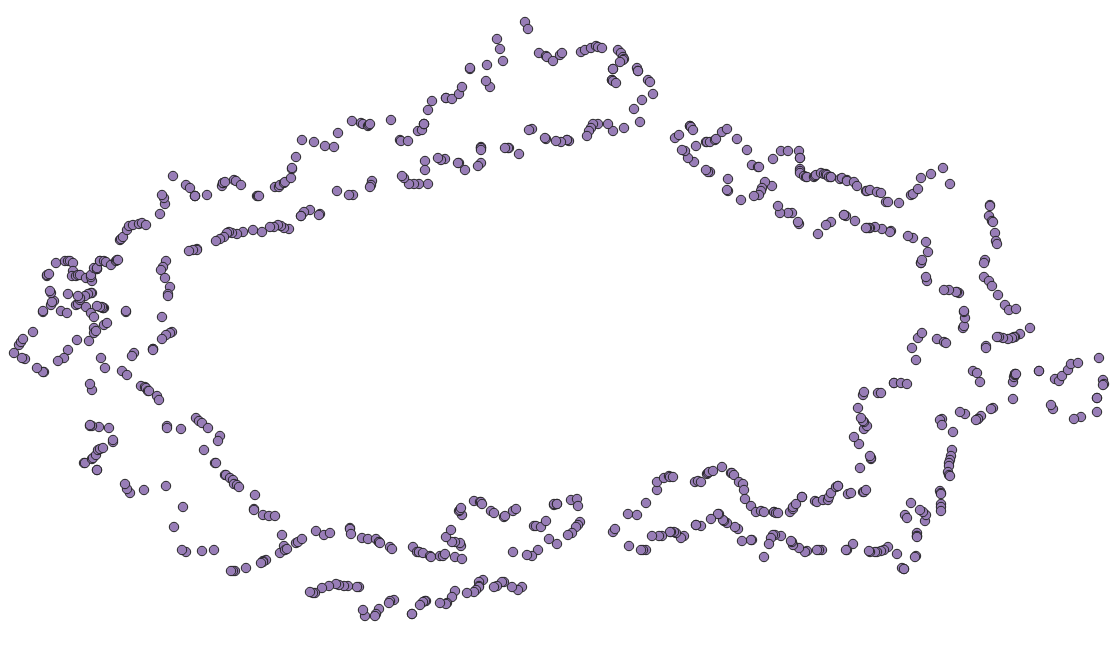
\includegraphics[width=400pt]{./pictures/vertices.png}
    \caption[Výsledek nástroje Extract vertices pro pásmo 2]{Výsledek nástroje Extract vertices pro pásmo 2}
	\label{fig:vertices}              
\end{figure} 

% ------- toto se nejspíš bude předělávat, jiná metoda řešení zastávek na hranici -------
Dále byly s pomocí třídy \textit{QgsVectorLayer} a její metody \textit{selectByExpression} vybrány 
z původní vektorové vrstvy \textit{stops} ty zastávky, které obsahovaly v poli \textit{zone\_id}
hodnotu tarifního pásma 1,2 nebo 2,3. Takové zastávky ležely na hranici pásma a polygon tarifního pásma
měl skrz ně vézt hranici. Z vybraných zastávek byla vytvořena vlastní vektorová vrstva. 
% ------- toto se nejspíš bude předělávat, jiná metoda řešení zastávek na hranici -------

Následně byly spojeny vektorové vrstvy hraniční zastávek, zastávek uvnitř tarifního pásma 2 a
bodů z výstupu nástroje \textit{Extract vertices} nástrojem \textit{Merge vector layers}.
Tyto tři zmiňované vektorové vrstvy byly vstupem do tohoto nástroje a výstupem byla 
vektorová vrstva spojených bodů. 

\begin{figure}[H] \centering
    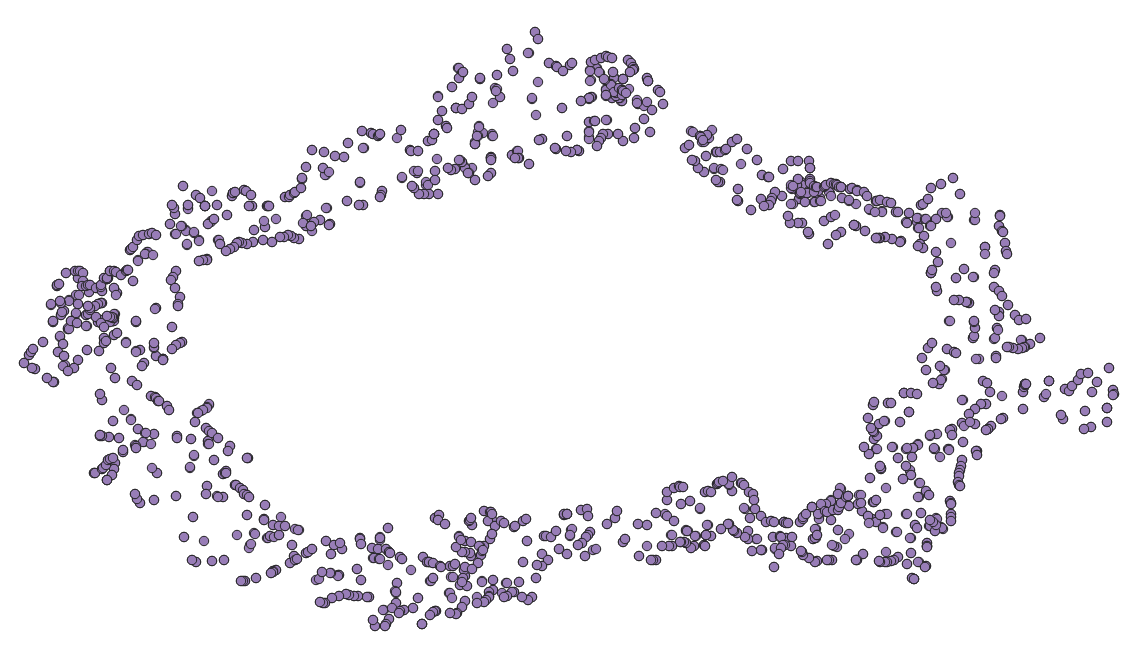
\includegraphics[width=400pt]{./pictures/merged.png}
    \caption[Spojené body třech vektorových vrstev pro pásmo 2]{Spojené body třech vektorových vrstev pro pásmo 2}
	\label{fig:merged}              
\end{figure} 

% Definice konkávní obálky 
Ze spojených bodů byla vytvořena konkávní obálka. To bylo provedeno nástrojem Concave hull (alpha shapes),
který počítá konkávní obálku z vstupních bodů. Vstupem tedy byla vrstva spojených bodů, což byl první parametr
nástroje. Dalším parametrem byl \textit{Práh (Threshold)} s datovým typem \textit{čísla}, který byl volen od 0 do 1,
kdy 0 znamenala maximum konkávní obálky a 1 konvexní obálky. Po několika testovacích spuštění byla 
určena hodnota 0,09 jako nejlepší hodnotou pro tvorbu tarifních pásem. Dalším parametrem bylo \textit{Povolení děr (Allow holes)} 
s datovým typem \textit{boolean}, který byl nastaven na \textit{False}.
Posledním parametrem bylo Rozdělit vícedílnou geometrii na jednotlivé části (Split multipart geometry 
into singlepart geometries) taktéž s datovým typem \textit{boolean}, který byl nastaven na \textit{True}.  
Výstupem byla polygonová vrstva konkávní obálky. 

\begin{figure}[H] \centering
    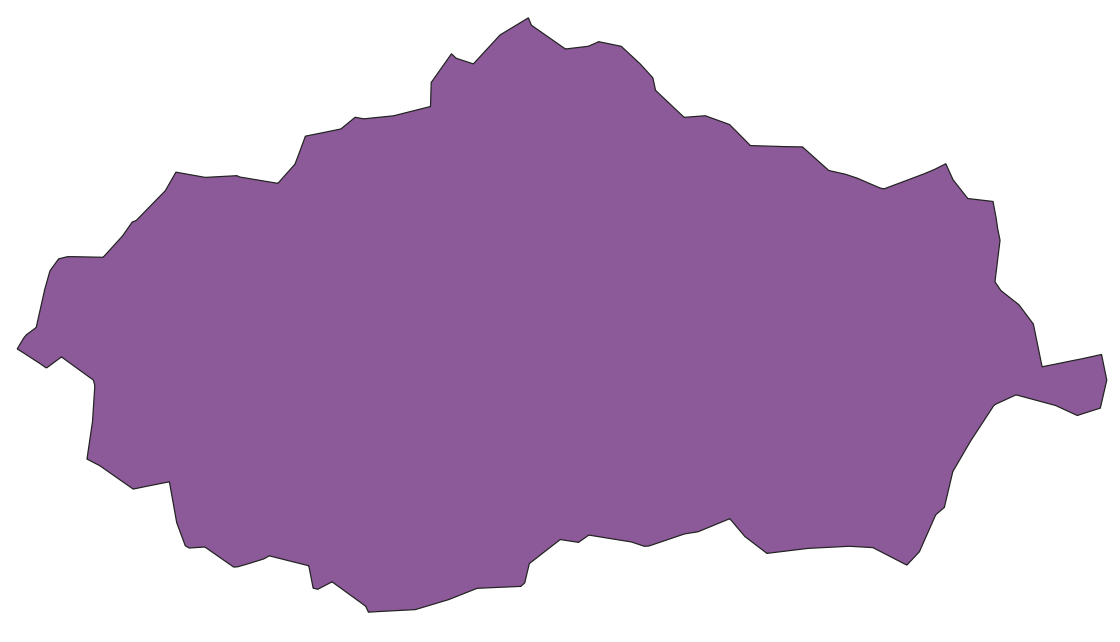
\includegraphics[width=400pt]{./pictures/concaveHull.png}
    \caption[Konkávní obálka pro pásmo 2]{Konkávní obálka pro pásmo 2}
	\label{fig:concaveHull}              
\end{figure} 

% Poté přes nástroj Select by location vyberu ty polygony, které se prostorově protínají (Intersect) se zastávkami v požadovaném tarifním pásmu. Nástroj Select by location funguje na bázi prostorových dotazů. Jeho zdrojový kód je opět veřejně publikován na GitHubu. Vstupem do tohoto nástroje je vektorová vrstva stops a vektorová vrstva Voroného polygonů. Jako příklad zde budu uvádět tarifní pásmo 2. 
% Je důležité si uvědomit, že jsem vybral ty Voroného polygony, které protínají zastávky s tarifním pásmem 2. Poté totiž existují takové zastávky, které leží na hranicích tarifních pásem. Takové zastávky mají hodnotu pole zone_id například 1,2 nebo 2,3. Typ pole zone_id je proto String. 
% Vybrané Voroného polygony poté nástrojem Dissolve spojím do jednoho uceleného polygonu (viz obr. 7). Vstupem pro tento nástroj jsou vybrané Voroného polygony. Jeho zdrojový kód je opět veřejně publikován na GitHubu. 
% Ze spojených polygonů poté nástrojem Extract vertices vygeneruji vektorovou vrstvu bodů (viz obr. 8), které představují vrcholy spojených polygonů. Zdrojový kód je opět na GitHubu.
% 
% Obr. 8 Vrcholy spojených polygonů tarifního pásma 2
% Dále s SQL dotazy vyberu z původní vrstvy stops ty body, které mají hodnotu tarifního pásma 2, vytvořím novou vektorovou vrstvu a stejně tak pro body, které jsou na hranicích a mají hodnotu tarifního pásma 1,2 nebo 2,3. Tyto dvě vektorové funkce se spojí do jedné vrstvy spolu s vrstvou z Extract vertices (viz obr. 9). 
% 
% Obr. 9 Všechny body zahrnující se do tarifního pásma 2
% Z těchto spojených bodů již už vytvářím konkávní obálku. Na tu jsou v QGISu taktéž nástroje, buď Concave hull (alpha shapes) nebo Concave hull (k-nearest neighbor). Vyzkoušel jsem oba nástroje, ale výsledky se od sebe tolik nelišily. Concave hull (alpha shapes) vytváří pomocí Delaunay triangulací trojúhelníky mezi jednotlivými body. Poté se vyhledávají nejdelší hrany trojúhelníků, který se při tom násobí s konstantou alpha (threshold), která se volí v rozmezí 0-1, kde 1 je už konvexní obálka. Z hran trojúhelníků vzniknou polygony a nakonec se nástrojem Dissolve tyto polygony zcelí. Volí se i parametr, zda jsou či nejsou povoleny díry v polygonech, kde jsem já zaškrtnul, že nejsou povoleny. Podrobný postup lze vyčíst opět ze zdrojového kódu, který je opět na GitHubu. Concave hull (k-nearest neighbor) má mnohem komplexnější postup a je k naleznutí opět na GitHubu. Ve zkratce tam hlavně závisí na počtu sousedních bodů, které je třeba vzít v úvahu (nižší počet je konkávnější, vyšší počet je hladší).
% Dále jsem na výsledek konkávní obálky použil nástroj Simplify. Algoritmus poskytuje výběr metod zjednodušení, včetně vzdálenosti založené (algoritmus „Douglas-Peucker“), založené na ploše (algoritmus „Visvalingam“) a přichytávání geometrií k mřížce. Já jsem volil první metodu založenou na algoritmu „Douglas-Peucker“. Jako parametr se také volí Tolerance ve stupních, která je závislá na souřadnicovém systému a na velikosti vstupních dat. Zdrojový kód je k naleznutí opět na GitHubu.
% Výsledek není moc patrný, tak by mohlo stát za uvážení tento krok přeskakovat.
% Dalším nástrojem je Smooth. Tento nástroj používá algoritmus Chaikin, který vyhlazuje geometrie v liniové nebo polygonové vrstvě. Vytvoří novou vrstvu s vyhlazenými geometriemi obsahujícími vyšší počet vrcholů a rohů v geometriích. Na vstupu jsou parametry jako počet iterací, offset – zlomek linie k vytvoření nových vrcholů podél, volí se mezi 0 a 1 (například výchozí hodnota 0,25 vytvoří nové vrcholy 25% a 75% podél každého liniového segmentu geometrie pro každou iteraci, menší hodnoty mají za následek „těsnější“ vyhlazení) a poslední parametr maximální úhel v uzlu (0 - 180), pod kterým bude provedeno vyhlazení. Zdrojový kód je k naleznutí opět na GitHubu.
% 
% Obr. 12 Výsledek nástroje Smooth - 10 iterací, 0.25 offset, 180 max úhel v uzlu
% 
% Tento postup se provedl ve smyčce pro každé tarifní pásmo zvlášť. Tarifní pásma P, B a 0 byly brány jako jedno pásmo. Poté se provedl rozdíl vrstev nástrojem Difference, aby se vzájemně nepřekrývaly. Také se smazaly „ostrovní“ polygony menší než 50 km2, které byly oddělené od těch primárních výsledných polygonů. Nakonec se tyto vektorové vrstvy spojily do jedné vrstvy (viz obr. 13).
% Pokud to porovnáme s obr. 3, tak si můžeme všimnout, že výsledek sice tuto vektorovou vrstvu připomíná, ale rozhodně není ideální. Čím se to počítá dále od středu, tak se tvoří horší podoby těchto pásem. Navíc v postupu není zakomponováno „vyhýbání se“ zastavěných oblastí, což je podmínka od pracovníků z ROPIDu.
% Problém s hraničními zastávkami
% Největší problém však vidím s tzv. hraničními zastávkami neboli zastávkami, které leží na hranicích jednotlivých pásem a skrz tyto zastávky musí hranice procházet. Jak lze vidět na obr. 14, obr. 15, obr. 16 (pro každý obrázek nahoře – můj výsledek, dole – výsledek ROPIDu), tak můj postup tento problém vůbec neřeší, proto ho volím jako nevhodný pro výsledek mé diplomové práce. V postupu by se musel vyřešit již u konkávní obálky (v Concave hull (alpha shapes) u Delaunay triangulace), kde by se musel přetvořit její algoritmus o „povinné body“, přes které by to navíc konkávní obálku počítalo. Avšak nic takového mě zatím nenapadlo a nevím, jestli to je vůbec možné.  
% 
% 

